% Options for packages loaded elsewhere
\PassOptionsToPackage{unicode}{hyperref}
\PassOptionsToPackage{hyphens}{url}
\PassOptionsToPackage{dvipsnames,svgnames,x11names}{xcolor}
%
\documentclass[
]{article}

\usepackage{amsmath,amssymb}
\usepackage{iftex}
\ifPDFTeX
  \usepackage[T1]{fontenc}
  \usepackage[utf8]{inputenc}
  \usepackage{textcomp} % provide euro and other symbols
\else % if luatex or xetex
  \usepackage{unicode-math}
  \defaultfontfeatures{Scale=MatchLowercase}
  \defaultfontfeatures[\rmfamily]{Ligatures=TeX,Scale=1}
\fi
\usepackage{lmodern}
\ifPDFTeX\else  
    % xetex/luatex font selection
    \setmainfont[]{Times New Roman}
\fi
% Use upquote if available, for straight quotes in verbatim environments
\IfFileExists{upquote.sty}{\usepackage{upquote}}{}
\IfFileExists{microtype.sty}{% use microtype if available
  \usepackage[]{microtype}
  \UseMicrotypeSet[protrusion]{basicmath} % disable protrusion for tt fonts
}{}
\makeatletter
\@ifundefined{KOMAClassName}{% if non-KOMA class
  \IfFileExists{parskip.sty}{%
    \usepackage{parskip}
  }{% else
    \setlength{\parindent}{0pt}
    \setlength{\parskip}{6pt plus 2pt minus 1pt}}
}{% if KOMA class
  \KOMAoptions{parskip=half}}
\makeatother
\usepackage{xcolor}
\setlength{\emergencystretch}{3em} % prevent overfull lines
\setcounter{secnumdepth}{-\maxdimen} % remove section numbering
% Make \paragraph and \subparagraph free-standing
\makeatletter
\ifx\paragraph\undefined\else
  \let\oldparagraph\paragraph
  \renewcommand{\paragraph}{
    \@ifstar
      \xxxParagraphStar
      \xxxParagraphNoStar
  }
  \newcommand{\xxxParagraphStar}[1]{\oldparagraph*{#1}\mbox{}}
  \newcommand{\xxxParagraphNoStar}[1]{\oldparagraph{#1}\mbox{}}
\fi
\ifx\subparagraph\undefined\else
  \let\oldsubparagraph\subparagraph
  \renewcommand{\subparagraph}{
    \@ifstar
      \xxxSubParagraphStar
      \xxxSubParagraphNoStar
  }
  \newcommand{\xxxSubParagraphStar}[1]{\oldsubparagraph*{#1}\mbox{}}
  \newcommand{\xxxSubParagraphNoStar}[1]{\oldsubparagraph{#1}\mbox{}}
\fi
\makeatother


\providecommand{\tightlist}{%
  \setlength{\itemsep}{0pt}\setlength{\parskip}{0pt}}\usepackage{longtable,booktabs,array}
\usepackage{calc} % for calculating minipage widths
% Correct order of tables after \paragraph or \subparagraph
\usepackage{etoolbox}
\makeatletter
\patchcmd\longtable{\par}{\if@noskipsec\mbox{}\fi\par}{}{}
\makeatother
% Allow footnotes in longtable head/foot
\IfFileExists{footnotehyper.sty}{\usepackage{footnotehyper}}{\usepackage{footnote}}
\makesavenoteenv{longtable}
\usepackage{graphicx}
\makeatletter
\newsavebox\pandoc@box
\newcommand*\pandocbounded[1]{% scales image to fit in text height/width
  \sbox\pandoc@box{#1}%
  \Gscale@div\@tempa{\textheight}{\dimexpr\ht\pandoc@box+\dp\pandoc@box\relax}%
  \Gscale@div\@tempb{\linewidth}{\wd\pandoc@box}%
  \ifdim\@tempb\p@<\@tempa\p@\let\@tempa\@tempb\fi% select the smaller of both
  \ifdim\@tempa\p@<\p@\scalebox{\@tempa}{\usebox\pandoc@box}%
  \else\usebox{\pandoc@box}%
  \fi%
}
% Set default figure placement to htbp
\def\fps@figure{htbp}
\makeatother

\makeatletter
\@ifpackageloaded{tcolorbox}{}{\usepackage[skins,breakable]{tcolorbox}}
\@ifpackageloaded{fontawesome5}{}{\usepackage{fontawesome5}}
\definecolor{quarto-callout-color}{HTML}{909090}
\definecolor{quarto-callout-note-color}{HTML}{0758E5}
\definecolor{quarto-callout-important-color}{HTML}{CC1914}
\definecolor{quarto-callout-warning-color}{HTML}{EB9113}
\definecolor{quarto-callout-tip-color}{HTML}{00A047}
\definecolor{quarto-callout-caution-color}{HTML}{FC5300}
\definecolor{quarto-callout-color-frame}{HTML}{acacac}
\definecolor{quarto-callout-note-color-frame}{HTML}{4582ec}
\definecolor{quarto-callout-important-color-frame}{HTML}{d9534f}
\definecolor{quarto-callout-warning-color-frame}{HTML}{f0ad4e}
\definecolor{quarto-callout-tip-color-frame}{HTML}{02b875}
\definecolor{quarto-callout-caution-color-frame}{HTML}{fd7e14}
\makeatother
\makeatletter
\@ifpackageloaded{caption}{}{\usepackage{caption}}
\AtBeginDocument{%
\ifdefined\contentsname
  \renewcommand*\contentsname{Table of contents}
\else
  \newcommand\contentsname{Table of contents}
\fi
\ifdefined\listfigurename
  \renewcommand*\listfigurename{List of Figures}
\else
  \newcommand\listfigurename{List of Figures}
\fi
\ifdefined\listtablename
  \renewcommand*\listtablename{List of Tables}
\else
  \newcommand\listtablename{List of Tables}
\fi
\ifdefined\figurename
  \renewcommand*\figurename{Figure}
\else
  \newcommand\figurename{Figure}
\fi
\ifdefined\tablename
  \renewcommand*\tablename{Table}
\else
  \newcommand\tablename{Table}
\fi
}
\@ifpackageloaded{float}{}{\usepackage{float}}
\floatstyle{ruled}
\@ifundefined{c@chapter}{\newfloat{codelisting}{h}{lop}}{\newfloat{codelisting}{h}{lop}[chapter]}
\floatname{codelisting}{Listing}
\newcommand*\listoflistings{\listof{codelisting}{List of Listings}}
\makeatother
\makeatletter
\makeatother
\makeatletter
\@ifpackageloaded{caption}{}{\usepackage{caption}}
\@ifpackageloaded{subcaption}{}{\usepackage{subcaption}}
\makeatother

\usepackage{bookmark}

\IfFileExists{xurl.sty}{\usepackage{xurl}}{} % add URL line breaks if available
\urlstyle{same} % disable monospaced font for URLs
\hypersetup{
  pdftitle={BÁO CÁO TUẦN 28 - NĂM 2025},
  colorlinks=true,
  linkcolor={blue},
  filecolor={Maroon},
  citecolor={Blue},
  urlcolor={Blue},
  pdfcreator={LaTeX via pandoc}}


\title{BÁO CÁO TUẦN 28 - NĂM 2025}
\author{}
\date{}

\begin{document}
\maketitle


\begin{minipage}[t]{0.48\textwidth}
\begin{center}
\textbf{TRUNG TÂM KIỂM SOÁT}\\
\textbf{BỆNH TẬT THÀNH PHỐ}\\
\underline{\textbf{KHOA GIÁM SÁT CẢNH BÁO,}}\\
\underline{\textbf{CHUẨN BỊ VÀ ĐÁP ỨNG KHẨN CẤP DỊCH BỆNH}}
\end{center}
\end{minipage}
\hfill
\begin{minipage}[t]{0.48\textwidth}
\begin{center}
\textbf{CỘNG HÒA XÃ HỘI CHỦ NGHĨA VIỆT NAM}\\
\textit{\textbf{Độc lập - Tự do - Hạnh phúc}}\\
\rule{5cm}{0.4pt}\\
TP. Hồ Chí Minh, ngày 25 tháng 7 năm 2025
\end{center}
\end{minipage}

\begin{tcolorbox}[enhanced jigsaw, leftrule=.75mm, opacityback=0, colframe=quarto-callout-color-frame, colback=white, rightrule=.15mm, bottomrule=.15mm, arc=.35mm, left=2mm, toprule=.15mm, breakable]

📥 Tải bản PDF của báo cáo này

\end{tcolorbox}

\section{I. Tình hình dịch bệnh sốt xuất huyết đến tuần
28:}\label{i.-tuxecnh-huxecnh-dux1ecbch-bux1ec7nh-sux1ed1t-xuux1ea5t-huyux1ebft-ux111ux1ebfn-tuux1ea7n-28}

\subsection{1. Đối với hoạt động giám sát dựa vào chỉ số
(IBS):}\label{ux111ux1ed1i-vux1edbi-houx1ea1t-ux111ux1ed9ng-giuxe1m-suxe1t-dux1ef1a-vuxe0o-chux1ec9-sux1ed1-ibs}

\begin{figure}[H]

{\centering \pandocbounded{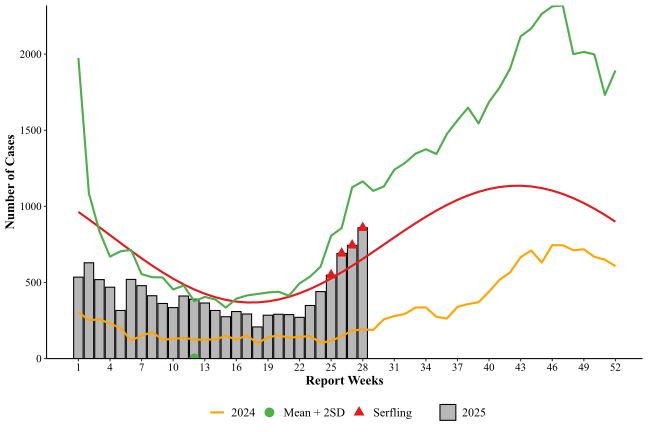
\includegraphics[keepaspectratio]{pic/serfling_sxh.png}}

}

\caption{Biểu đồ 1: Diễn tiến dịch sốt xuất huyết đến tuần 28/2025}

\end{figure}%

Trong tuần 28/2025, trên toàn Thành phố ghi nhận được 859 ca mắc mới,
tăng khoảng 15,4\% so với tuần trước và tăng khoảng 41,8\% so với trung
bình 4 tuần trước. Tính từ đầu năm, số ca tích lũy đến tuần 28 ghi nhận
được 11.911 ca, tăng khoảng 167,9\% so với cùng kì năm trước.

Diễn tiến số ca mắc sốt xuất huyết từ đầu năm đến nay nằm dưới ngưỡng
(Trung bình + 2 lần Độ lệch chuẩn). Tuy nhiên, theo phương pháp cảnh báo
Serfling, số ca vượt ngưỡng từ tuần 25 và xu hướng cảnh báo liên tục đến
tuần hiện tại.

\subsection{2. Đối với hoạt động giám sát dựa vào sự kiện
(EBS):}\label{ux111ux1ed1i-vux1edbi-houx1ea1t-ux111ux1ed9ng-giuxe1m-suxe1t-dux1ef1a-vuxe0o-sux1ef1-kiux1ec7n-ebs}

\subsubsection{a. Kết quả giám sát xu hướng tìm kiếm thông tin dịch bệnh
truyền nhiễm qua nền tảng Google Trends (Công cụ giám sát Google
Trends):}\label{a.-kux1ebft-quux1ea3-giuxe1m-suxe1t-xu-hux1b0ux1edbng-tuxecm-kiux1ebfm-thuxf4ng-tin-dux1ecbch-bux1ec7nh-truyux1ec1n-nhiux1ec5m-qua-nux1ec1n-tux1ea3ng-google-trends-cuxf4ng-cux1ee5-giuxe1m-suxe1t-google-trends}

- Mức độ quan tâm:

- Từ khóa hàng đầu (top queries):

- Từ khóa gia tăng (top rising):

\subsubsection{b. Kết quả giám sát các trang tin điện tử, báo chí liên
quan đến dịch BTN, sự kiện y tế công cộng (công cụ Media
scanning):}\label{b.-kux1ebft-quux1ea3-giuxe1m-suxe1t-cuxe1c-trang-tin-ux111iux1ec7n-tux1eed-buxe1o-chuxed-liuxean-quan-ux111ux1ebfn-dux1ecbch-btn-sux1ef1-kiux1ec7n-y-tux1ebf-cuxf4ng-cux1ed9ng-cuxf4ng-cux1ee5-media-scanning}

\begin{longtable}[]{@{}lllll@{}}
\caption{*Ghi chú: CIR-Critical Information Reporting -- Sự kiện quan
trọng, khẩn cấp cần phải báo cáo ngay}\tabularnewline
\toprule\noalign{}
Ngày thu thập & TP.HCM & Tỉnh khác & Nước ngoài & Thuộc CIR \\
\midrule\noalign{}
\endfirsthead
\toprule\noalign{}
Ngày thu thập & TP.HCM & Tỉnh khác & Nước ngoài & Thuộc CIR \\
\midrule\noalign{}
\endhead
\bottomrule\noalign{}
\endlastfoot
07/7/2025 & 0 & 0 & 2 & 0 \\
08/7/2025 & 0 & 0 & 0 & 0 \\
09/7/2025 & 0 & 0 & 0 & 0 \\
10/7/2025 & 0 & 0 & 0 & 0 \\
11/7/2025 & 0 & 0 & 0 & 0 \\
Tổng & 0 & 0 & 0 & 0 \\
Thuộc CIR & 0 & 1 & 0 & 0 \\
\end{longtable}

\section{II. Tình hình dịch bệnh tay chân miệng đến tuần
28:}\label{ii.-tuxecnh-huxecnh-dux1ecbch-bux1ec7nh-tay-chuxe2n-miux1ec7ng-ux111ux1ebfn-tuux1ea7n-28}

\subsection{1. Đối với hoạt động giám sát dựa vào chỉ số
(IBS):}\label{ux111ux1ed1i-vux1edbi-houx1ea1t-ux111ux1ed9ng-giuxe1m-suxe1t-dux1ef1a-vuxe0o-chux1ec9-sux1ed1-ibs-1}

\begin{figure}[H]

{\centering \pandocbounded{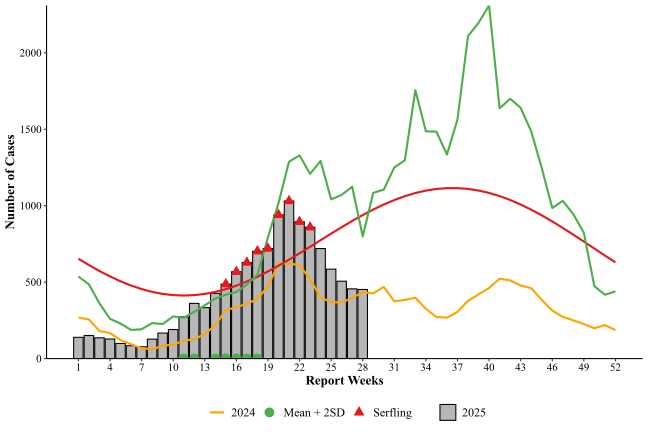
\includegraphics[keepaspectratio]{pic/serfling_tcm.png}}

}

\caption{Biểu đồ 2: Diễn tiến dịch tay chân miệng đến tuần 28/2025}

\end{figure}%

Trong tuần 28/2025, trên toàn Thành phố ghi nhận được 452 ca mắc mới,
giảm khoảng 0,8\% so với tuần trước và tăng khoảng 20,2\% so với trung
bình 4 tuần trước. Tính từ đầu năm, số ca tích lũy đến tuần 28 ghi nhận
được 12.241 ca, tăng khoảng 48,7\% so với cùng kì năm trước.

Đối với cảnh báo sớm, số ca bệnh đã vượt ngưỡng trung bình cộng 2 lần độ
lệch chuẩn từ tuần 14 đế tuần 18. Tuy nhiên, phương pháp Serfling cảnh
báo số ca tăng bất thường từ tuần 15 và cảnh báo liên tục đến tuần 23.
Số ca bệnh trong tuần 28 đã giảm dưới ngưỡng của 2 phương pháp cảnh báo
dịch.

\subsection{2. Đối với hoạt động giám sát dựa vào sự kiện
(EBS):}\label{ux111ux1ed1i-vux1edbi-houx1ea1t-ux111ux1ed9ng-giuxe1m-suxe1t-dux1ef1a-vuxe0o-sux1ef1-kiux1ec7n-ebs-1}

\subsubsection{a. Kết quả giám sát xu hướng tìm kiếm thông tin dịch bệnh
truyền nhiễm qua nền tảng Google Trends (Công cụ giám sát Google
Trends):}\label{a.-kux1ebft-quux1ea3-giuxe1m-suxe1t-xu-hux1b0ux1edbng-tuxecm-kiux1ebfm-thuxf4ng-tin-dux1ecbch-bux1ec7nh-truyux1ec1n-nhiux1ec5m-qua-nux1ec1n-tux1ea3ng-google-trends-cuxf4ng-cux1ee5-giuxe1m-suxe1t-google-trends-1}

- Mức độ quan tâm:

- Từ khóa hàng đầu (top queries):

- Từ khóa gia tăng (top rising):

\subsubsection{b. Kết quả giám sát các trang tin điện tử, báo chí liên
quan đến dịch BTN, sự kiện y tế công cộng (công cụ Media
scanning):}\label{b.-kux1ebft-quux1ea3-giuxe1m-suxe1t-cuxe1c-trang-tin-ux111iux1ec7n-tux1eed-buxe1o-chuxed-liuxean-quan-ux111ux1ebfn-dux1ecbch-btn-sux1ef1-kiux1ec7n-y-tux1ebf-cuxf4ng-cux1ed9ng-cuxf4ng-cux1ee5-media-scanning-1}

\begin{longtable}[]{@{}lllll@{}}
\caption{*Ghi chú: CIR-Critical Information Reporting -- Sự kiện quan
trọng, khẩn cấp cần phải báo cáo ngay}\tabularnewline
\toprule\noalign{}
Ngày thu thập & TP.HCM & Tỉnh khác & Nước ngoài & Thuộc CIR \\
\midrule\noalign{}
\endfirsthead
\toprule\noalign{}
Ngày thu thập & TP.HCM & Tỉnh khác & Nước ngoài & Thuộc CIR \\
\midrule\noalign{}
\endhead
\bottomrule\noalign{}
\endlastfoot
07/7/2025 & 0 & 0 & 2 & 0 \\
08/7/2025 & 0 & 0 & 0 & 0 \\
09/7/2025 & 0 & 0 & 0 & 0 \\
10/7/2025 & 0 & 0 & 0 & 0 \\
11/7/2025 & 0 & 0 & 0 & 0 \\
Tổng & 0 & 0 & 0 & 0 \\
Thuộc CIR & 0 & 1 & 0 & 0 \\
\end{longtable}

\section{Nhận định}\label{nhux1eadn-ux111ux1ecbnh}

\section{Đề xuất}\label{ux111ux1ec1-xuux1ea5t}




\end{document}
